\RequirePackage{silence}
\WarningFilter{hyperref}{Token not allowed}
\WarningFilter{microtype}{tracking amount}
\WarningFilter{chessfss}{\comment already}
% LaTeX: More Than Just Academic Papers and Journals
%
% Copyright Lim Lian Tze 2011-2016 (liantze@gmail.com) 
% Beamer presentation slides for a talk at the Malaysian Open Source Conference 
% 2011 (MOSC 2011 http://www.mosc.my/)
%
% http://liantze.penguinattack.org/latextypesetting.html
%
% This work is licensed under a Creative Commons Attribution-NonCommercial-
% ShareAlike 3.0 Unported License (http://creativecommons.org/licenses/by-nc-sa/3.0/).
%

%\pdfminorversion=5
%\pdfobjcompresslevel=3 
%\pdfcompresslevel=9

% Full presentation (with overlays, animated bullet items etc)
\documentclass[aspectratio=169,xcolor={x11names,svgnames,dvipsnames}]{beamer}

% Transparency mode (no overlays)
%\documentclass[xcolor={x11names,svgnames,dvipsnames},trans]{beamer}

% n-up handout mode
% \documentclass[xcolor={x11names,svgnames,dvipsnames},handout]{beamer}

\usepackage{pgfpages}
\usepackage{qrcode}

\usepackage[british]{babel}
\usepackage[utf8]{inputenc}
\usepackage[T1]{fontenc}
\usepackage{lmodern}
% \usepackage[linesnumbered,lined,commentsnumbered]{algorithm2e}
\usepackage[lined]{algorithm2e}
\usepackage{graphicx}

%% Glossy pretty look for the presentation and transparency (w/o overlays and animations) versions!
\mode<beamer|trans>{
\useoutertheme[glossy]{wuerzburg}
\useinnertheme[shadow,outline]{chamfered}
\usecolortheme{shark}
}
\setbeamertemplate{navigation symbols}{}
\setbeamertemplate{frametitle continuation}[from second][(cont'd)]
\usefonttheme[stillsansseriftext,stillsansserifsmall]{serif}

%% Save up on ink for the 4-up handouts
\mode<handout>{
\useoutertheme{wuerzburg}
\useinnertheme[outline]{chamfered}
%\pgfpagesuselayout{4 on 1}[a4paper, landscape, border shrink=10mm]
\pgfpagesuselayout{2 on 1}[a4paper, border shrink=10mm]
\pgfpageslogicalpageoptions{1}{border code=\pgfstroke}
\pgfpageslogicalpageoptions{2}{border code=\pgfstroke}
%\pgfpageslogicalpageoptions{3}{border code=\pgfstroke}
%\pgfpageslogicalpageoptions{4}{border code=\pgfstroke}
\setbeamercolor{structure}{fg=black}
\setbeamercolor{alerted text}{fg=black}
}

\mode<presentation>{\AtBeginSection[]{%
\begin{frame}
\frametitle{Contents}
\tableofcontents[currentsection]
\end{frame}}}

\usepackage[T1,safe]{tipa}
\usepackage{microtype}
\usepackage[utf8]{inputenc}
\usepackage[T1]{fontenc}
\usepackage{libertine}
\usepackage[scaled=.77]{beramono}
\SetTracking{encoding=*}{-39}

\usepackage{relsize,tabularx}
\usepackage{hologo,textcomp}
\usepackage{comment}
\usepackage[skaknew]{chessboard,skak}
\usepackage{multicol,booktabs}
\usepackage{listings}
\lstset{upquote,keepspaces=true,columns=spaceflexible,
basicstyle=\ttfamily\scriptsize,%
breaklines=true,breakindent=0pt,xleftmargin=0pt, xrightmargin=6pt,%
language=[LaTeX]TeX, texcsstyle=*\bfseries\color{Maroon}, commentstyle=\sffamily\itshape\smaller\color{SeaGreen4},
emphstyle=\bfseries\color{RoyalBlue3},escapechar={:},
emphstyle={[2]{\bfseries\color{Sienna2}}},
postbreak=\mbox{{\smaller\color{gray}$\hookrightarrow$}}
}

\mode<handout>{
   \lstset{
   texcsstyle=*\bfseries, commentstyle=\sffamily\itshape\smaller,
   emphstyle=\bfseries,escapechar={:},
   emphstyle={[2]{\bfseries}},
   emphstyle={[3]{\bfseries}},
   postbreak=\mbox{{\smaller$\hookrightarrow$}}
   }
}

\makeatletter
\lst@CCPutMacro\lst@ProcessOther {"2D}{\lst@ttfamily{-{}}{-{}}}
\@empty\z@\@empty
\makeatother


\usepackage{tikz}
\usepackage{pgfgantt}
\usetikzlibrary{shapes,arrows,positioning,matrix,chains,fit}
\usetikzlibrary{backgrounds}

\usepackage[caption=false,font=footnotesize]{subfig}
\usepackage{blindtext}
\usepackage{amssymb}
\usepackage{amsthm}
\usepackage{amsmath}
\usepackage{mathtools}
\usepackage{changepage}
\usepackage{color}
\usepackage{colortbl}
\usepackage{hhline}
\usepackage{array}
\usepackage{multicol,multirow}
\usepackage[version=3]{mhchem}
\usepackage{chemfig}
\usepackage{expex,qtree}
% \usepackage{texshade}
\usepackage[detect-all]{siunitx}
% \usepackage[siunitx]{circuitikz}
\usepackage{smartdiagram}
\usepackage{bytefield}
\usepackage{fancybox}
\usepackage{graphicx}
\usepackage{color}
\usepackage{epsfig}

\usepackage{epstopdf}
\usepackage{multimedia}
%\usepackage[latin1]{inputenc}
%\usepackage{indentfirst}
%\usepackage[brazil]{babel}
\usepackage{mdframed}
\usepackage{multirow}
\usepackage{booktabs}
\usepackage{epstopdf}
\usepackage{xspace}
\bibliographystyle{unsrt}
% \usepackage{pstricks,pst-barcode}
% \usepackage{auto-pst-pdf}

\definecolor{light-gray}{rgb}{0.98, 0.99, 0.99}
\definecolor{light-orange}{rgb}{0.95, 0.95, 0.99}
\definecolor{light-green}{rgb}{0.90,0.95,0.90}
\definecolor{sepia}{rgb}{0.44, 0.26, 0.08}
\definecolor{olive}{rgb}{0.5, 0.5, 0.0}
\definecolor{safe1}{rgb}{0.38, 0.38, 0.38}
\definecolor{safe2}{rgb}{0.74, 0.74, 0.74}
\definecolor{safe3}{rgb}{0.90, 0.90, 0.90}
%\definecolor{ceruleanblue}{rgb}{0.16, 0.32, 0.75}
%\definecolor{cornellred}{rgb}{0.7, 0.11, 0.11}
%\definecolor{darkpastelgreen}{rgb}{0.01, 0.75, 0.24}
%\definecolor{green(pigment)}{rgb}{0.0, 0.65, 0.31}




\newcolumntype{L}{>{\scriptsize}l}
\newcolumntype{C}{>{\scriptsize}c} % define a new column type for \tin

\newcolumntype{x}{>{\columncolor{light-gray}}C}
\newcolumntype{y}{>{\columncolor{white}}C}
\newcolumntype{z}{>{\columncolor{light-orange}}C}


\usepackage{pgfplots}
\pgfplotsset{compat=1.12}
\usepackage{cwpuzzle}
\usepackage{gchords,guitar}
\usepackage{spreadtab}
\usepackage{ccicons}
\usepackage{marvosym}
\usepackage{upgreek}
\usepackage{adforn}
% \ifpdf
\pdfmapfile{+webo.map}
% \fi
\newcommand{\wb}[1]{{\usefont{U}{webo}{xl}{n}#1}}
\usepackage{bookmark}

\usepackage{graphicx}

\usepackage{epigraph}
\setlength{\epigraphwidth}{1\textwidth}

\setlength\fboxsep{0pt}


\author[Rafael Diniz]{\texorpdfstring{\textcolor{blue}{Rafael Diniz} \\
{Rhizomatica} \\
{HERMES - High-frequency Emergency and Rural Multimedia Exchange System}\\
\url{rafael@rhizomatica.org}}{Rafael Diniz}}
\title{Long-range Telecommunications in the HF band}
\subtitle{
\texorpdfstring{ %(\textsc{UT--Dallas})\\%
\hrulefill\ \adforn{57}\thickspace\wb{.}\thickspace\adforn{29}\ \hrulefill}
%{First Presented at MOSC 2011; some modifications since}
}

\titlegraphic{
\includegraphics[width=.4\textwidth]{logo.png} \ \ \ \ \ \ \  \\}
\date[15-Feb-2023]{OsmoDevCall, February, 2023}
\hypersetup{%
pdfauthor={Rafael Diniz}, %% the "author" field from above includes garbage code...
%pdfkeywords={latex,features,publicity,preview}
}
\begin{document}

\begin{frame}[plain]
\maketitle
\end{frame}


\begin{frame}
\begin{center}
  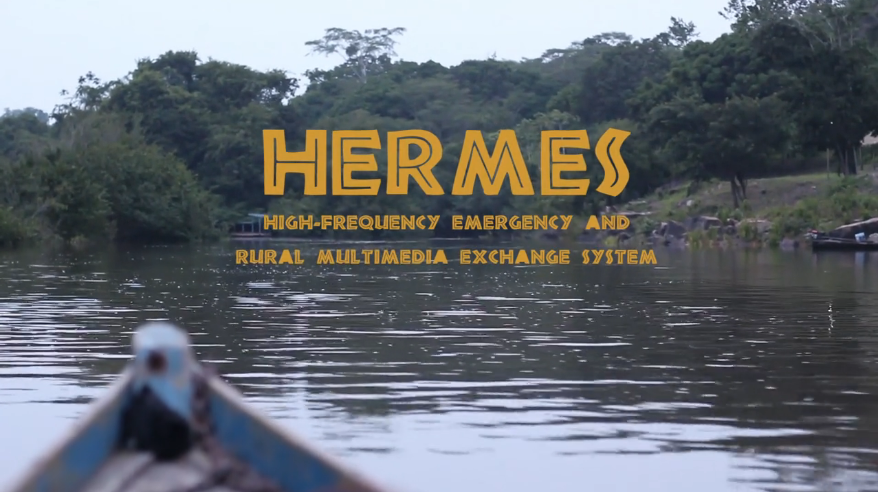
\includegraphics[width=.9\columnwidth]{hermes.png}
\end{center}
\end{frame}


\begin{frame}{HERMES}

\begin{center}
%  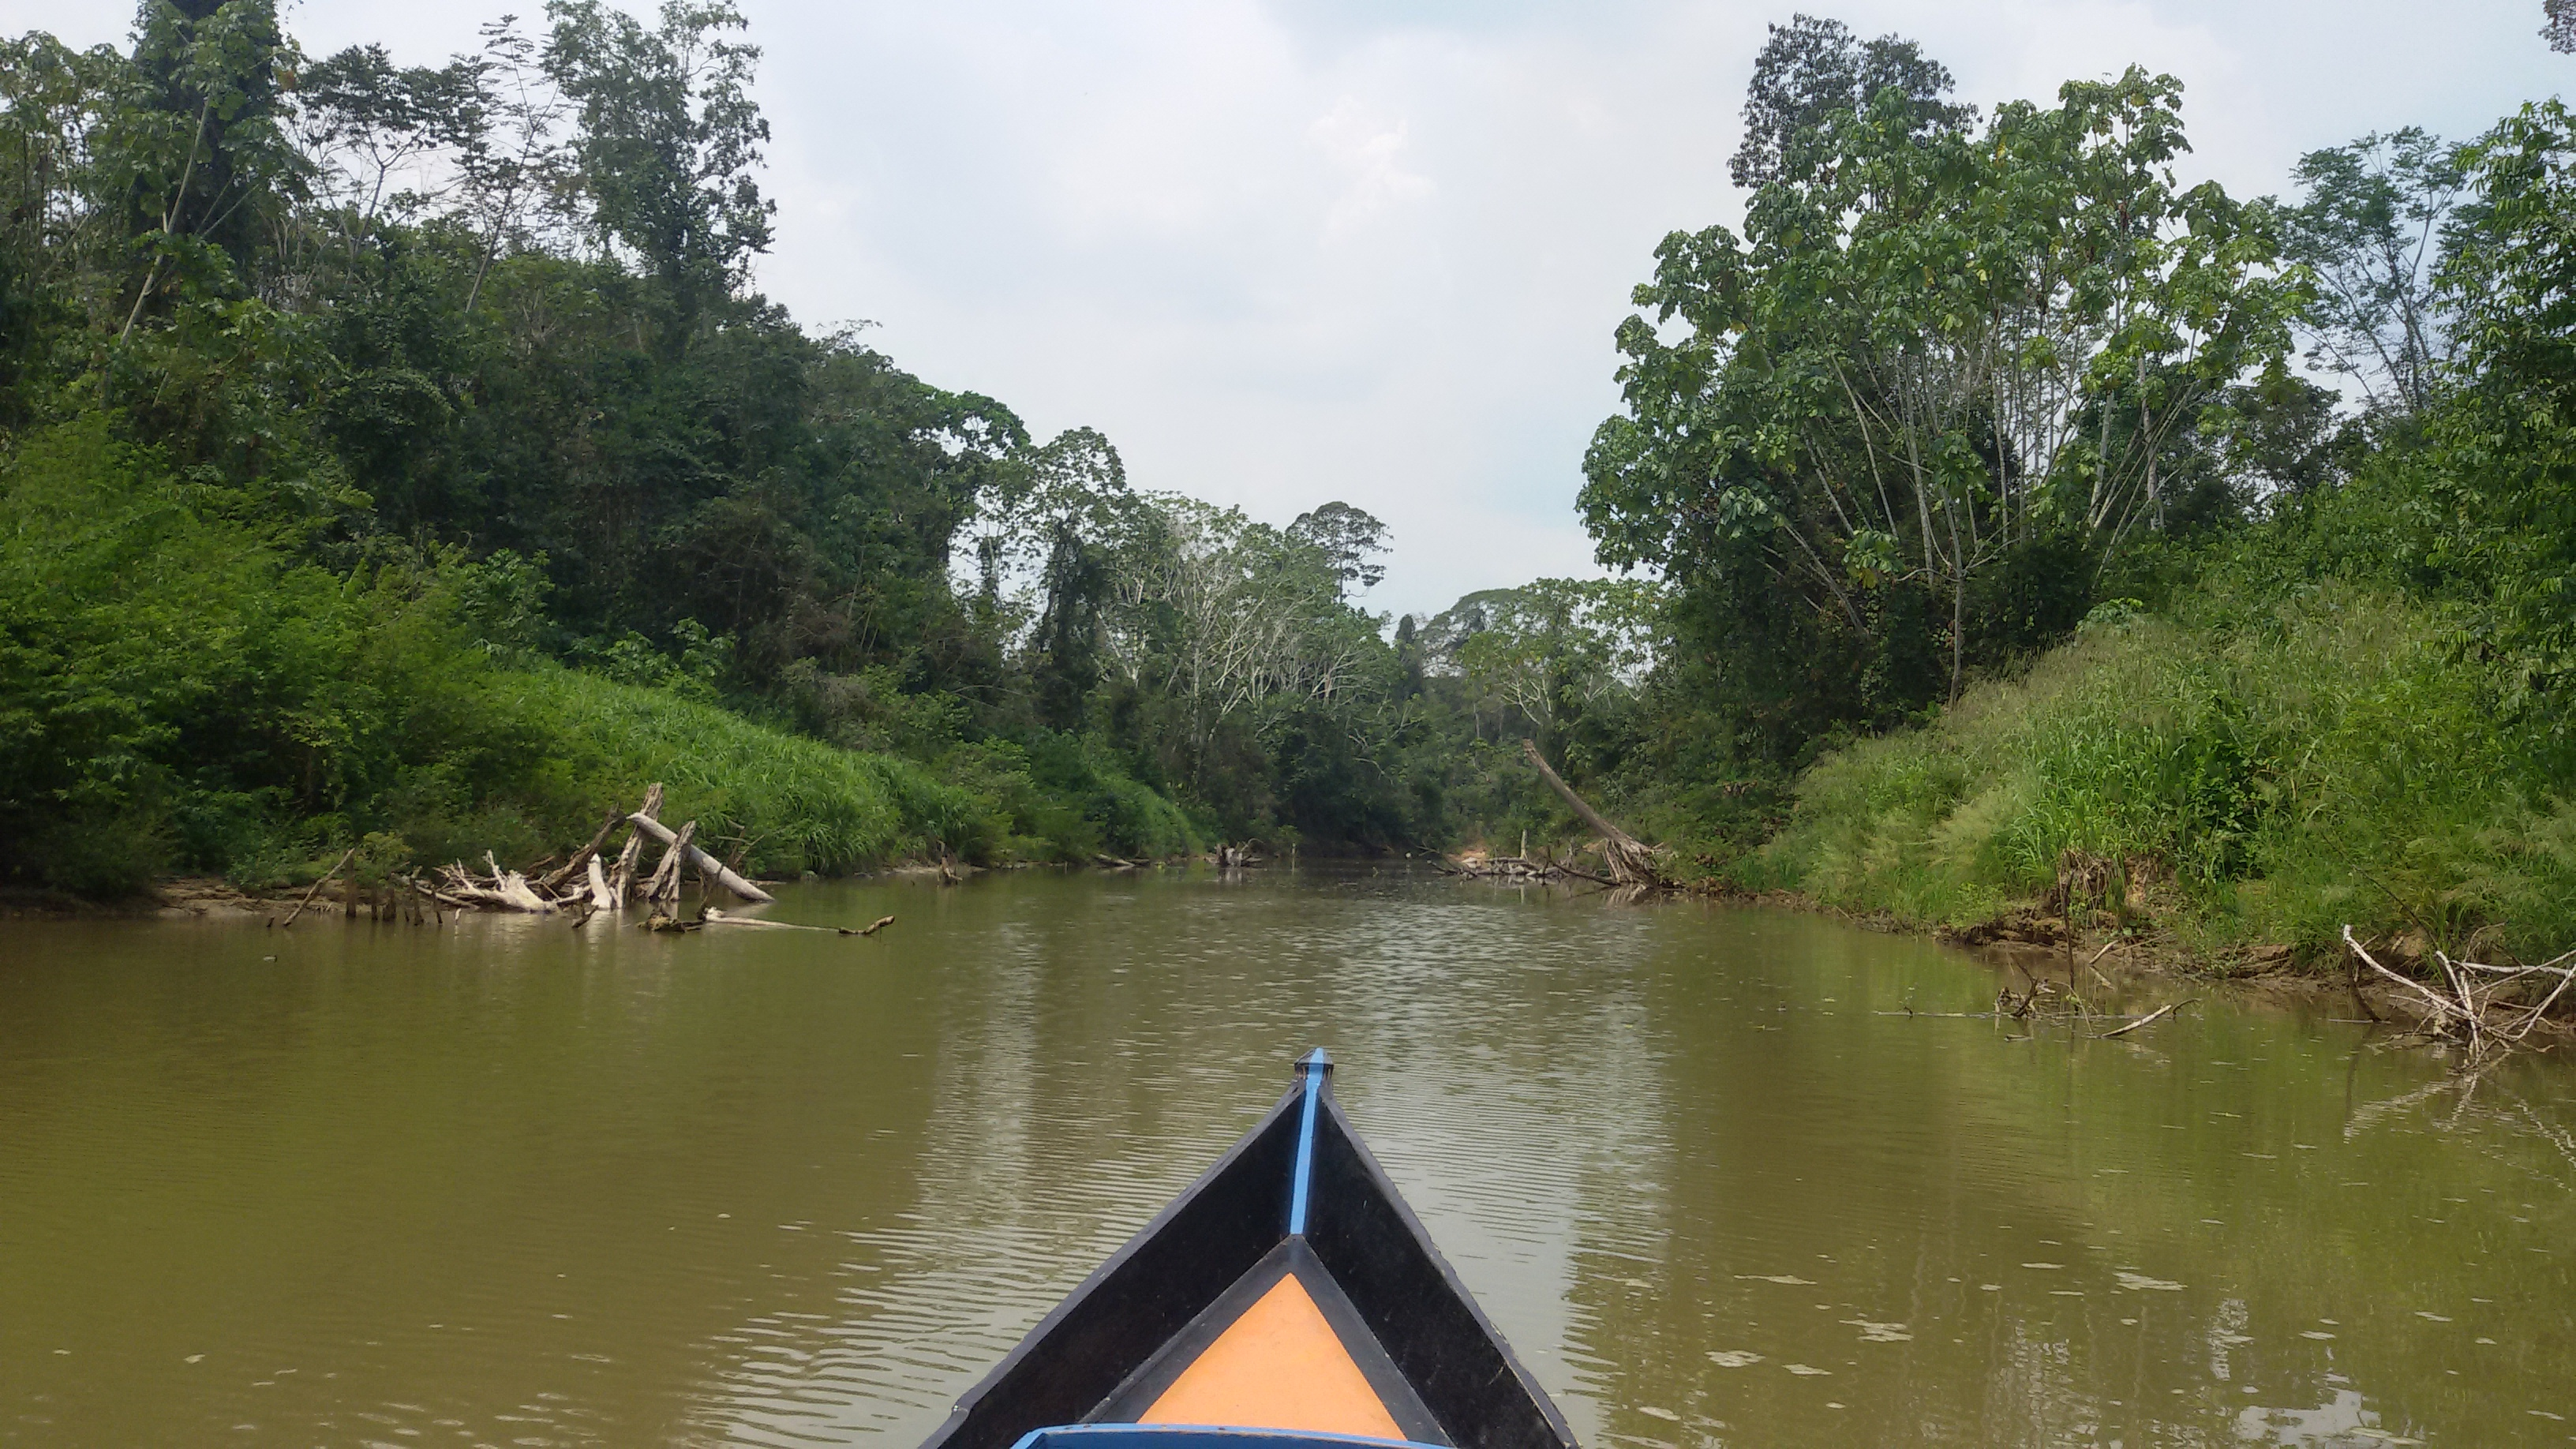
\includegraphics[width=.45\columnwidth]{boat.jpg}
  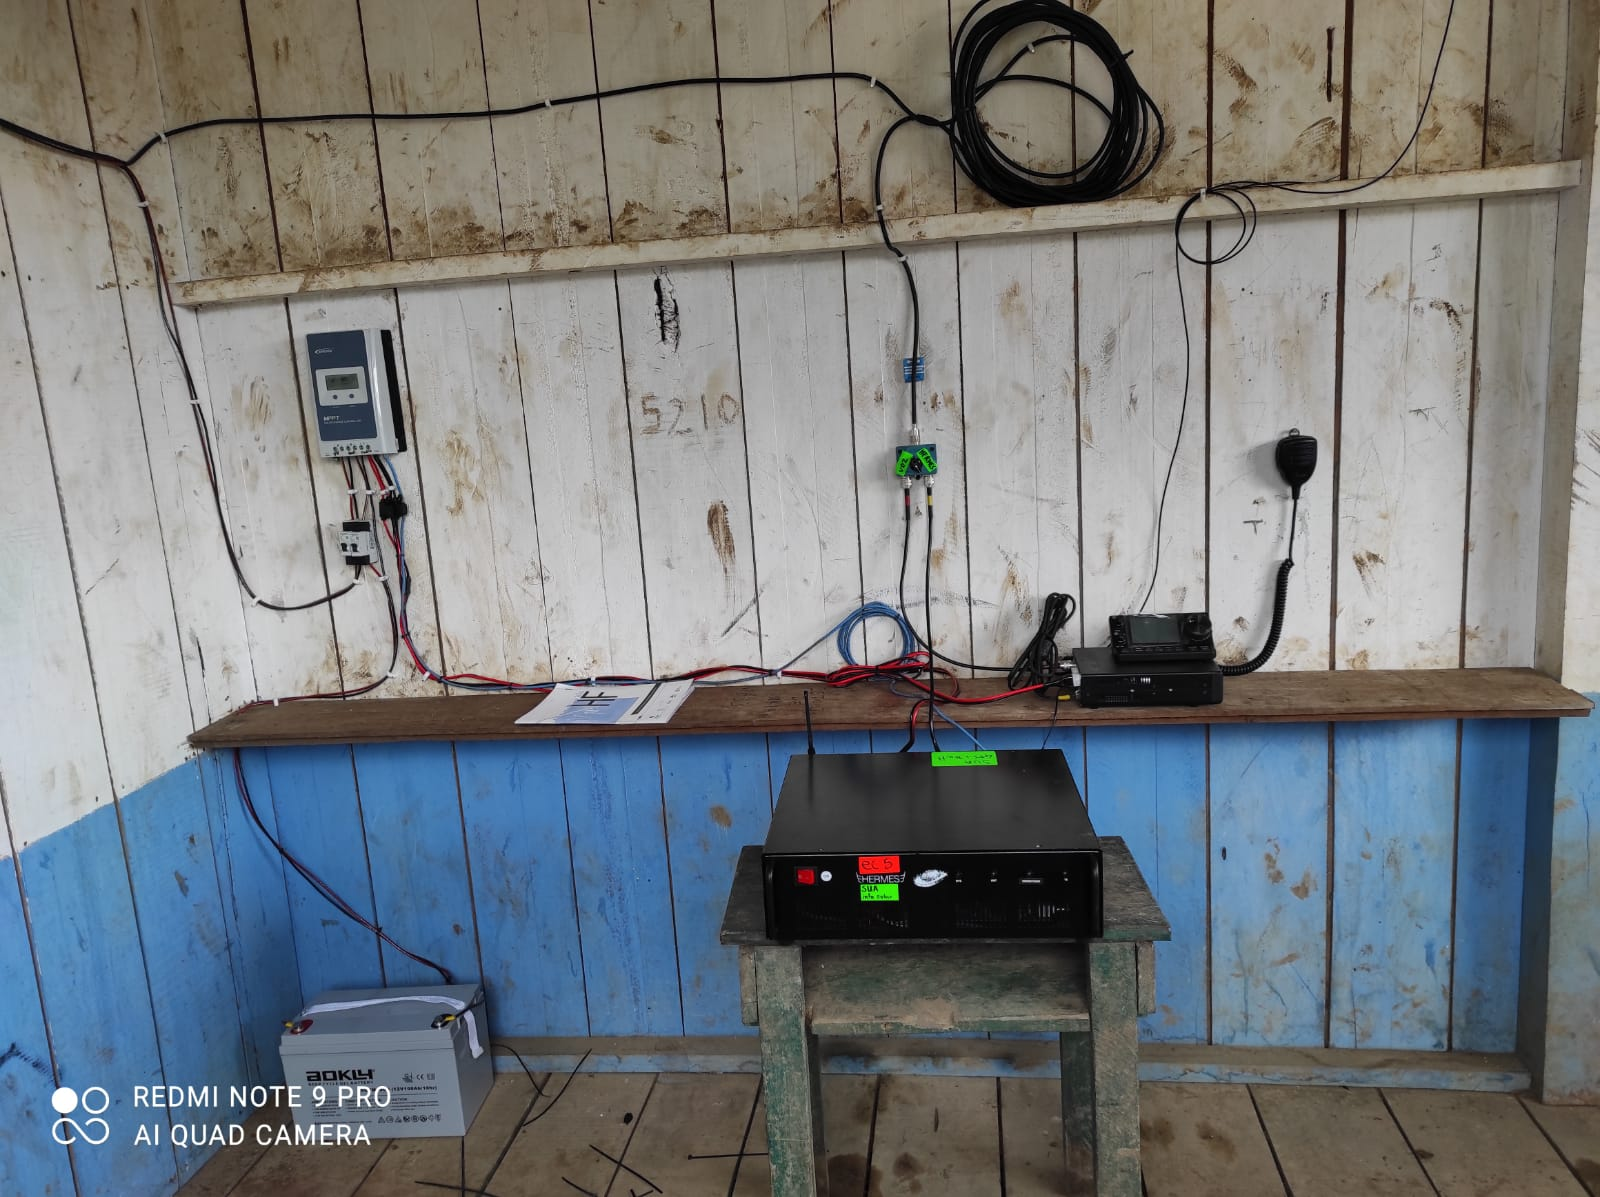
\includegraphics[width=.7\columnwidth]{hermes.jpeg}
\end{center}

\end{frame}

\begin{frame}{HERMES}

\begin{center}
%  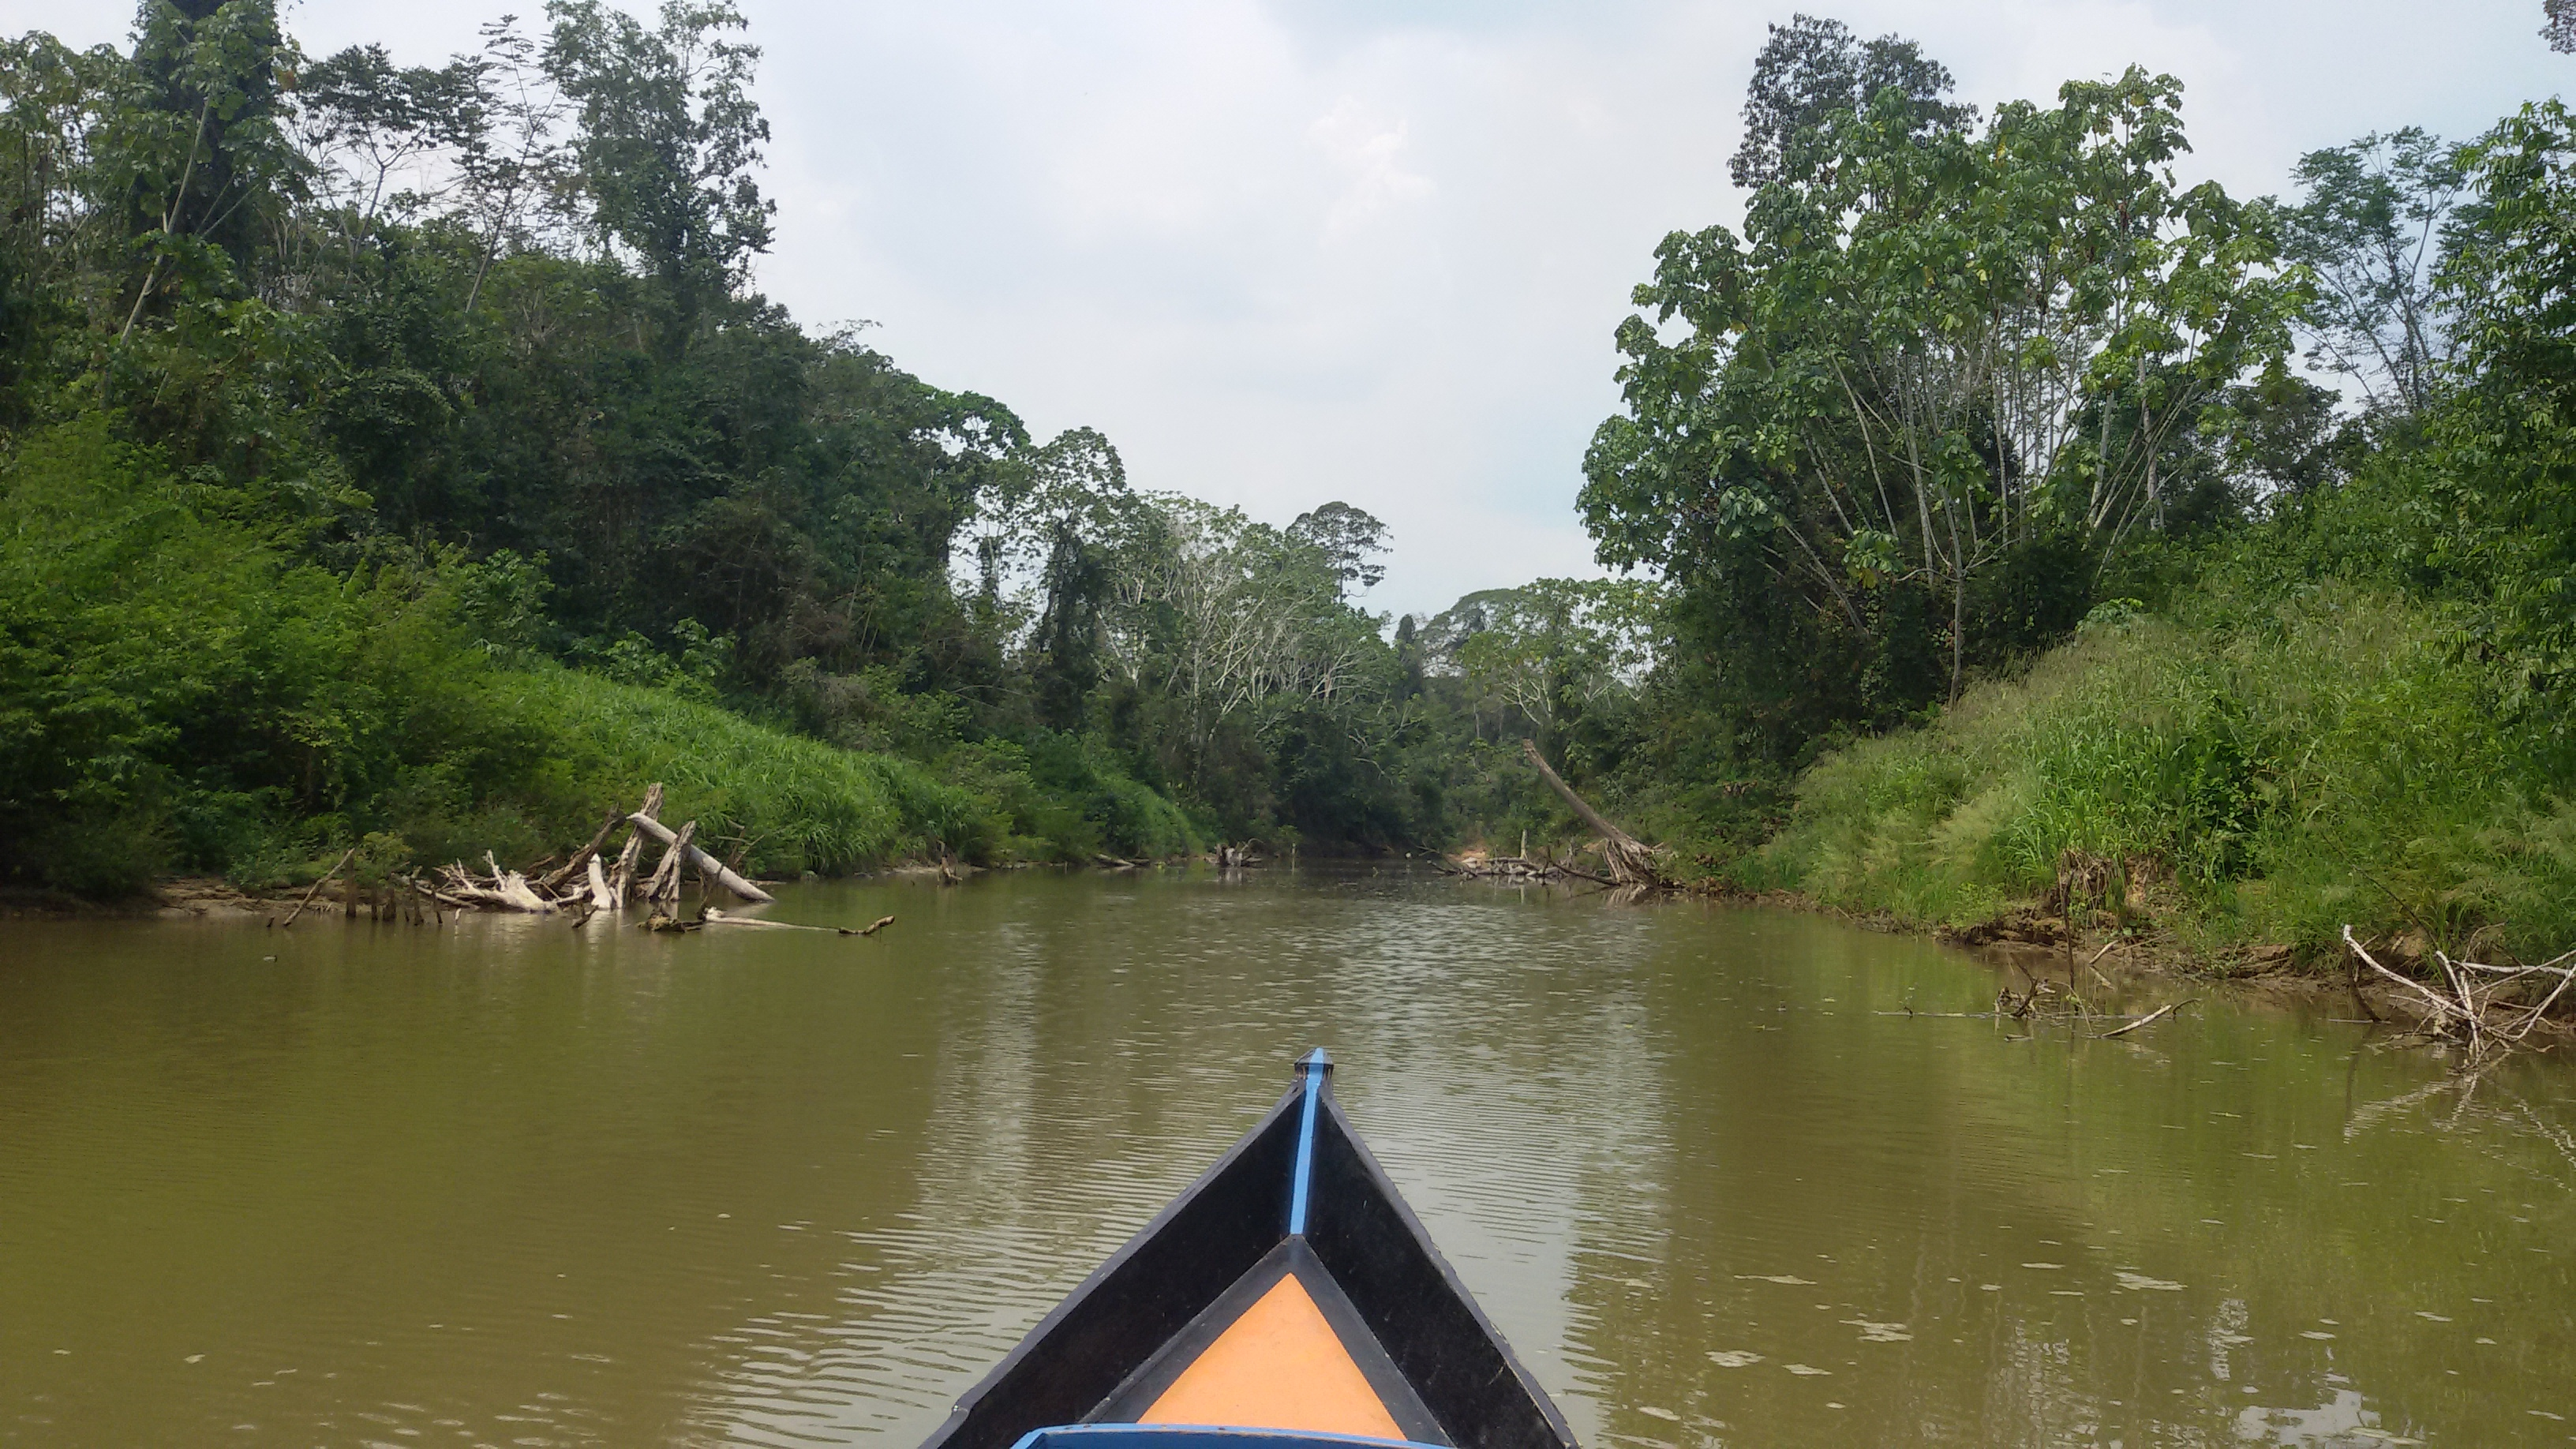
\includegraphics[width=.45\columnwidth]{boat.jpg}
  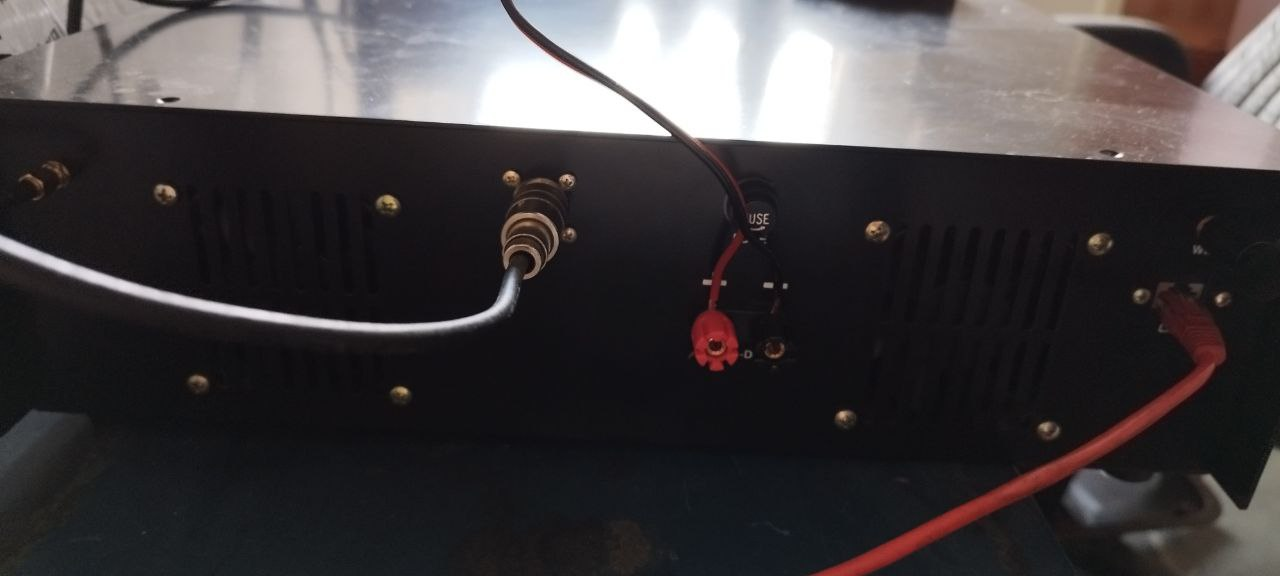
\includegraphics[width=.95\columnwidth]{hermes-back.jpeg}
\end{center}

\end{frame}


% Slide 2
\begin{frame}{The HF Band}

  \begin{itemize}
    \item The band, as defined by ITU, between 3 MHz and 30 MHz
    \item The HF band allows very wide coverage thanks to the skywave propagation
    \item Civil HF telecommunication systems are stuck on time (around the 60's)
    \item Military HF telecommunication systems are very advanced, already in its 4G era (aka. WideBand ALE)
  \end{itemize}

\begin{center}
  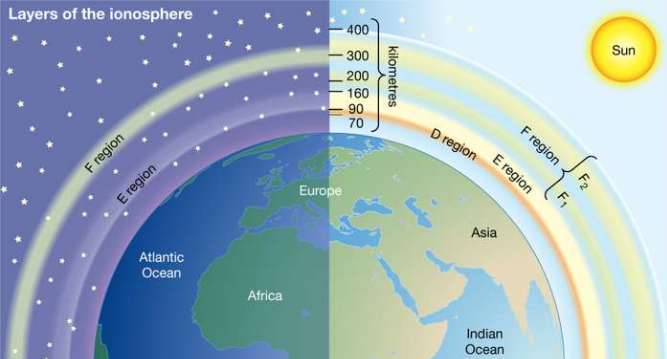
\includegraphics[width=.45\columnwidth]{ionosfera.png}
\end{center}

\end{frame}

% Slide 2
\begin{frame}{Real-world network example}

  \begin{itemize}
  \item In the Amazon rainforest regin, Pará state, northern Brazil
  \end{itemize}

\begin{center}
  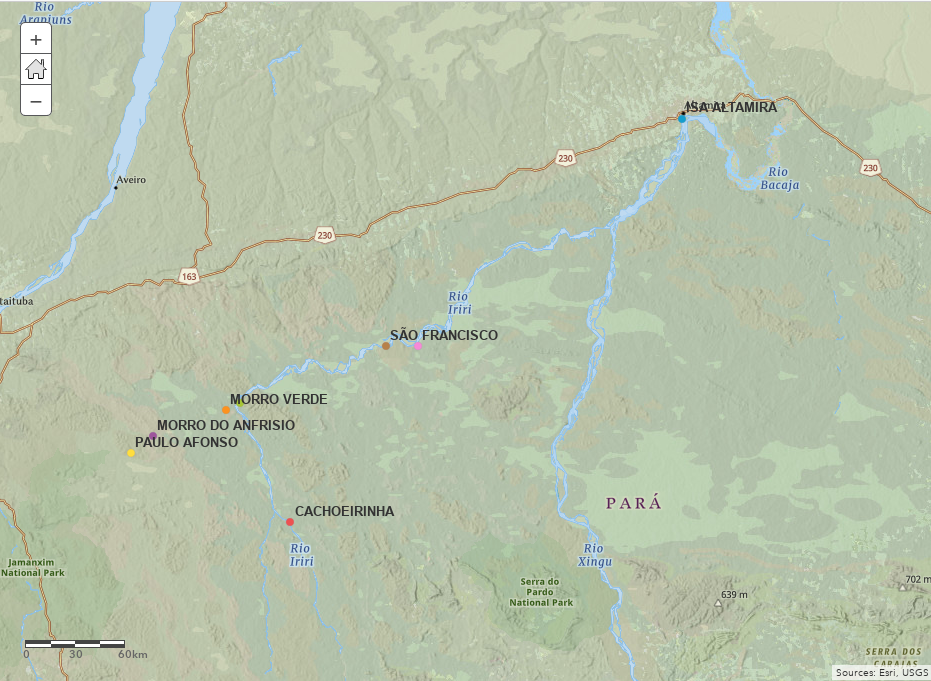
\includegraphics[width=.57\columnwidth]{radio_stations.png}
\end{center}

\end{frame}

\begin{frame}{Antenna}
    \begin{center}
      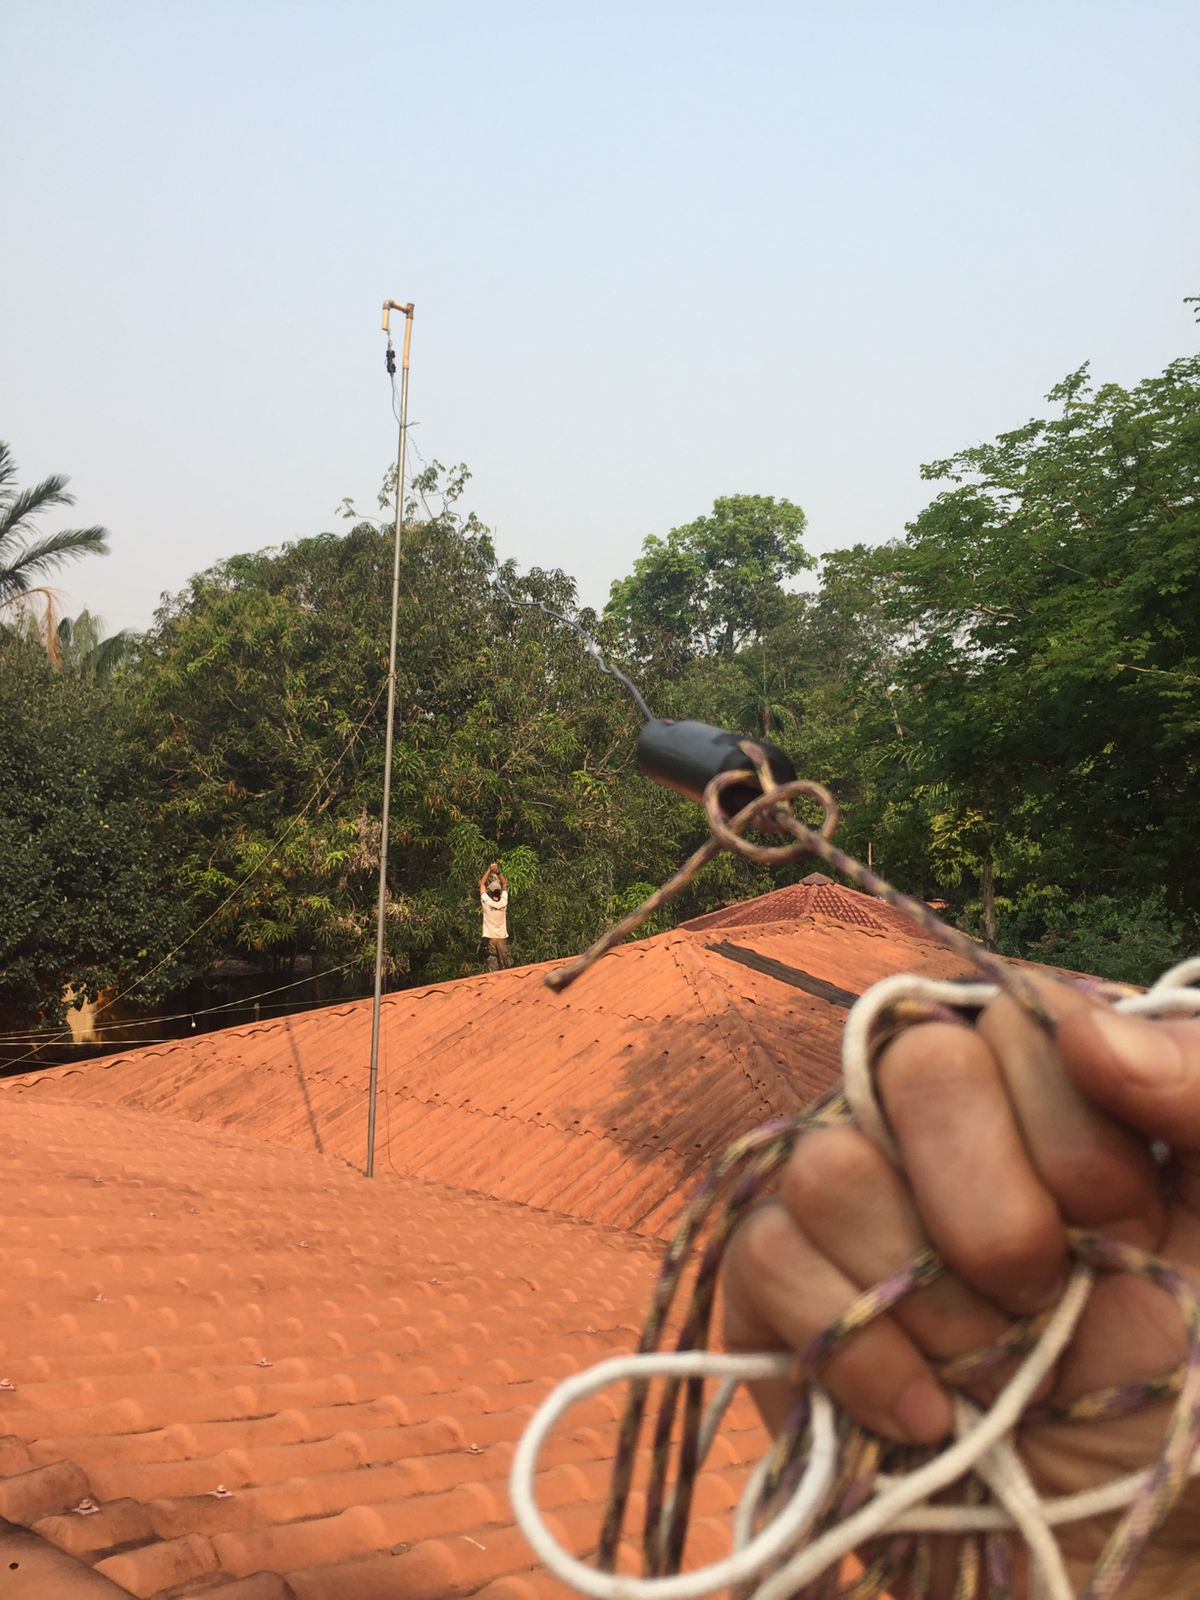
\includegraphics[width=.5\columnwidth]{antena.jpeg}
    \end{center}
\end{frame}

\begin{frame}{System Description}
      \begin{itemize}
      \item HF Transceiver
      \item UUCP-based Network Stack (x86 PC)
      \item User-facing services
      \end{itemize}

%    \begin{center}
      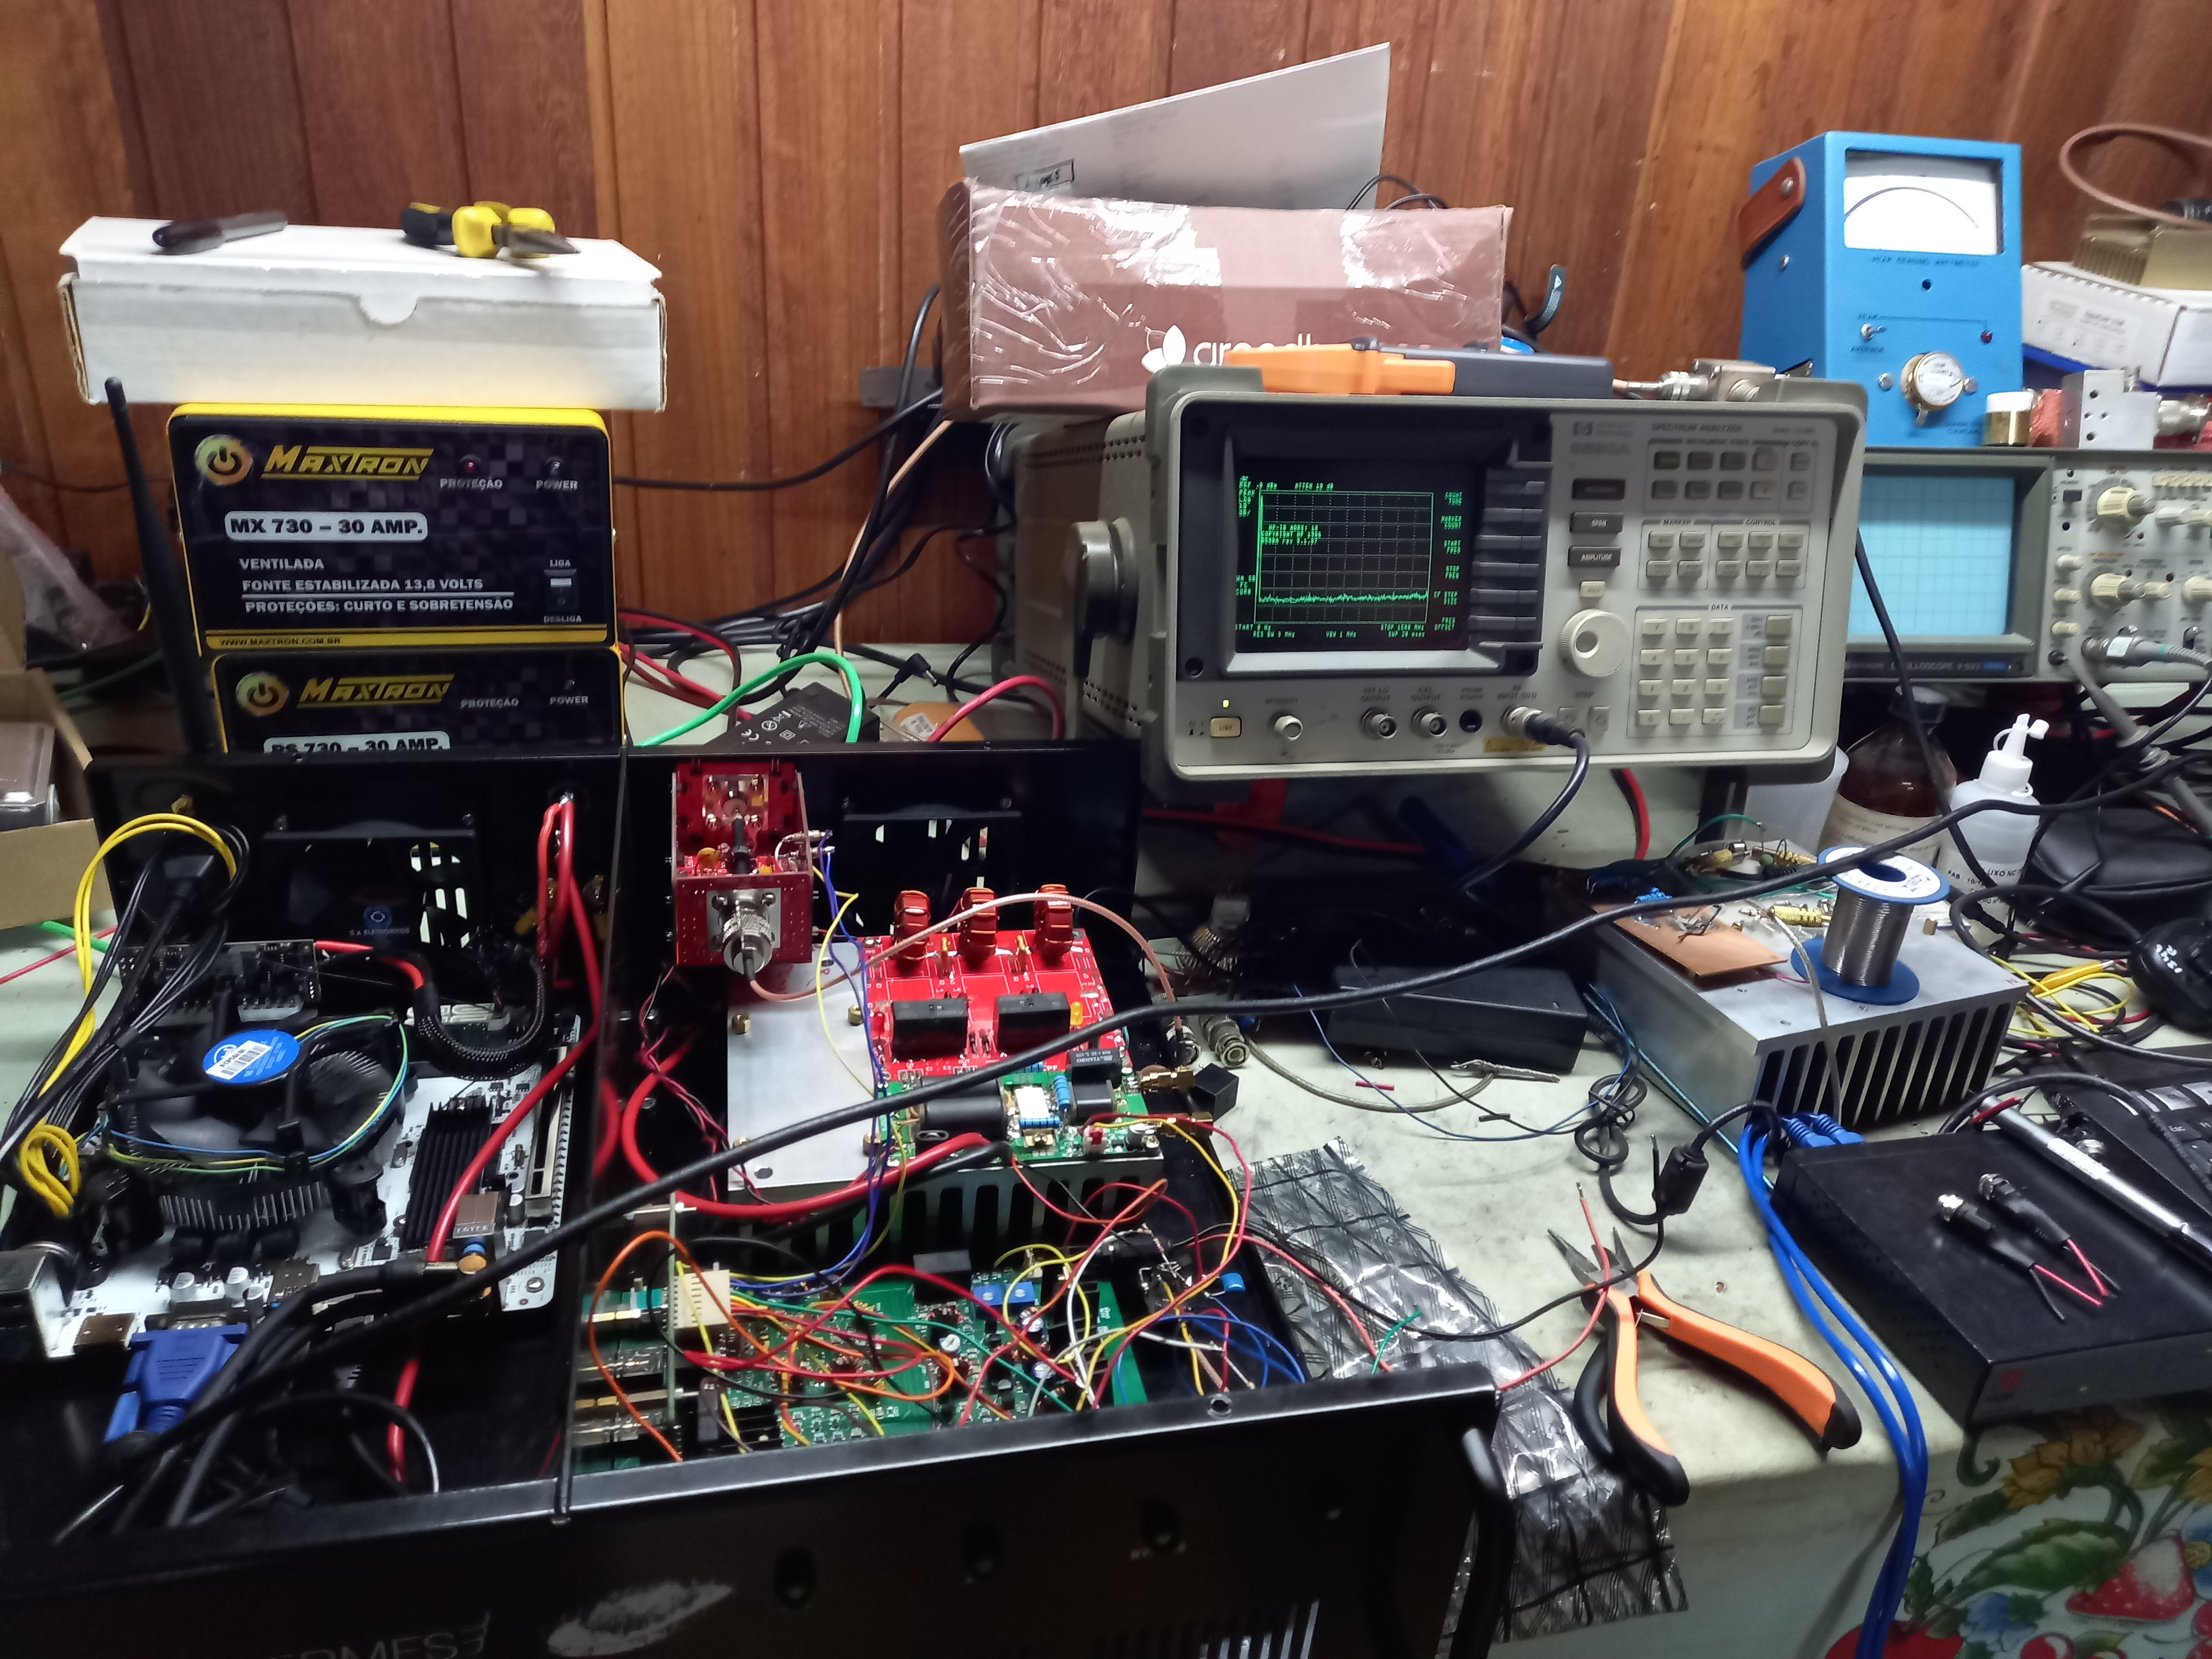
\includegraphics[width=.4\columnwidth]{pic3.jpg} 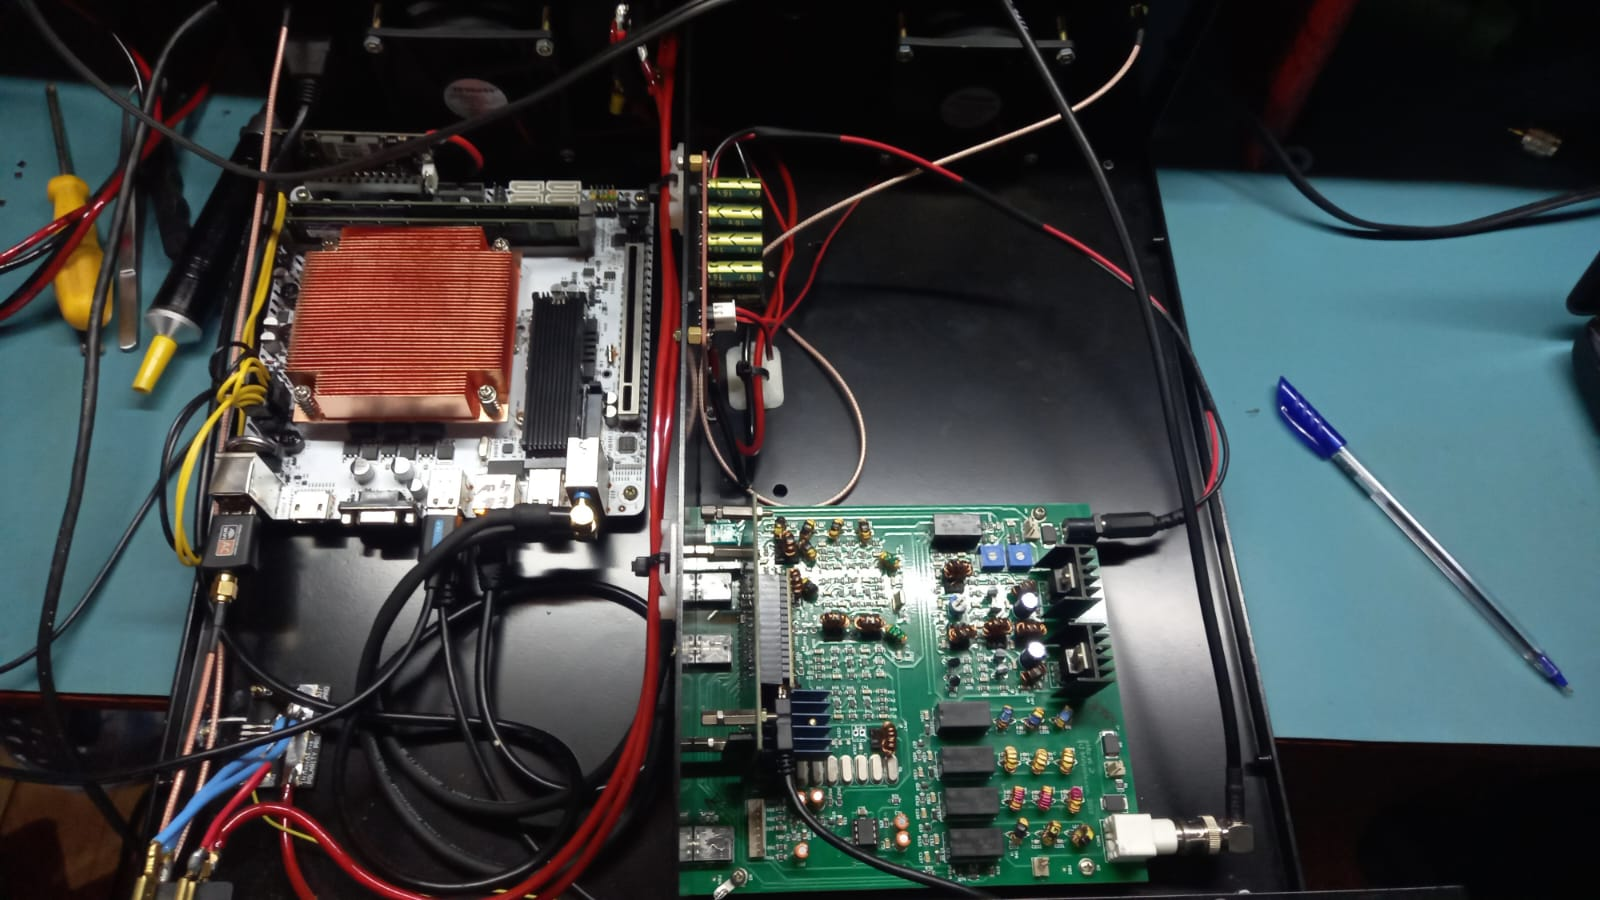
\includegraphics[width=.49\columnwidth]{hermes2.jpeg}

%    \end{center}

\end{frame}

\begin{frame}{HF transceiver}

  \begin{center}
https://www.hfsignals.com/index.php/ubitx-v6-buy-the-full-kit/
  \end{center}

\begin{block}{µBitx v6 based}
    \begin{itemize}
    \item Arduino firmware re-written, includes a new serial communication protocol, LEDs control...
    \item Added a GPS for calibration of the PLL offset (Si5351A)
    \item Added a lambda bridge for forward and reflected power measurement
    \end{itemize}
  \end{block}

\begin{center}
  \vspace{-0.5cm}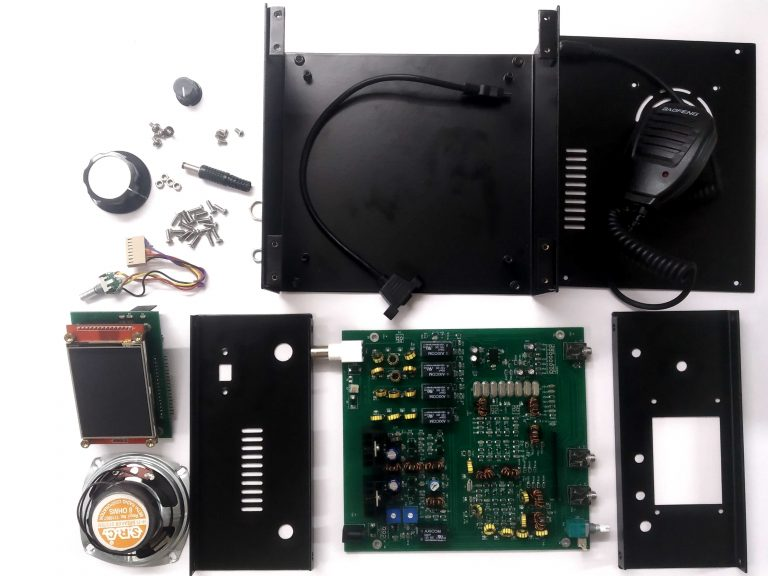
\includegraphics[width=.35\columnwidth]{ubitx.jpg}
\end{center}

\end{frame}


\begin{frame}{(software-defined) Modem}

\begin{block}{Currently using VARA HF}
    \begin{itemize}
    \item 2300 Hz BW, ARQ, Adaptive Modulation
    \item Modes range from 16 bps up to 5 kbps
    \item Proprietary Visual Basic 6 application (runs well on Wine)
    \end{itemize}
  \end{block}

\begin{center}
  \vspace{-0.15cm}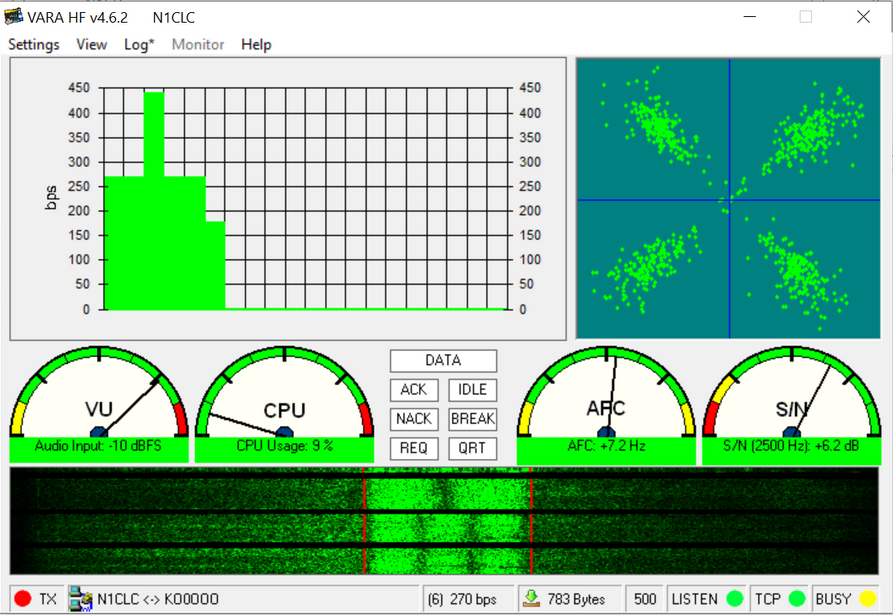
\includegraphics[width=.42\columnwidth]{vara.png}
\end{center}

\end{frame}


\begin{frame}{New Modem}

\begin{block}{We are developing Mercury modem}
    \begin{itemize}
    \item Flexible BW (including wideband waveforms greater than 3 kHz)
    \item Uses OFDM modulation and LDPC
    \item https://github.com/Rhizomatica/mercury
    \end{itemize}
  \end{block}

  \begin{center}
    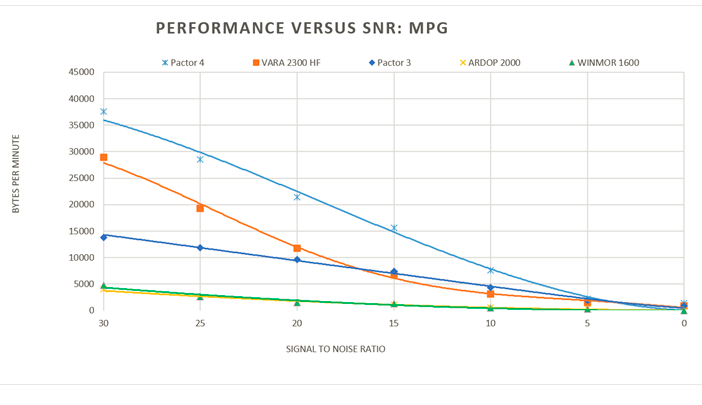
\includegraphics[width=.55\columnwidth]{image_modems.png}
  \end{center}

\end{frame}

\begin{frame}{Good ol' UUCP}

\begin{block}{Taylor's UUCP goes over the air}
    \begin{itemize}
    \item UUCP connects to the modem using pipes and shared memory
    \item The UUCP nodename is the station callsign
    \item Is composed by a daemon which transfers the uucp payload between uucico and the HF modem.
    \item Protocol 'y' is used, and long timeouts are set.
    \end{itemize}
  \end{block}

/etc/uucp/port:
\vspace{0.5cm}

port HFP
\\
type pipe\\
command /usr/bin/uuport -c \textbackslash Z

\end{frame}

\begin{frame}{The network stack (hermes-net repo)}

\begin{block}{https://github.com/Rhizomatica/hermes-net}
    \begin{itemize}
    \item trx\_v1-firmware: The HF transceiver firmware
    \item trx\_v1-userland: radio control daemon and cli tool
    \item uucpd: UUCP daemon and tools (bridge between UUCP and the modem)
    \item uuxcomp: uux wrapper which compresses an e-mail before enqueuing it, and crmail to decompress
    \item system\_scripts: image and audio compression scripts, email and uucp management, gateway ``caller'', etc
    \item system\_services: init scripts and udev rules
    \end{itemize}
  \end{block}

\end{frame}


\begin{frame}{REST Backend}

\begin{block}{https://github.com/Rhizomatica/hermes-api}
    \begin{itemize}
    \item Radio API: set/get frequency, mode, bfo, pll offset, pwr ref, fwd, swr, ...
    \item User API: user management for web admin access and e-mail accounts (same login)
    \item Messages API: direct message between hosts (just a uucp copy of a packaged message)
    \item System API: set/get system status / configuration
    \item UUCP API: provides a way to list and delete UUCP jobs, and start a connection (uucico)
    \item Special Gateway API: provides scheduling facitities and station/frequency table
    \end{itemize}
  \end{block}

\end{frame}

\begin{frame}{WEB Frontend}

\begin{block}{https://github.com/Rhizomatica/hermes-gui}
  \begin{itemize}
  \item Provides users Web access to the needed configurations
  \item Multi-language: en, es, pt
  \item System logs, UUCP queue management
  \item Message writing / received / transmitted messages
  \item User management is tied to email user management
  \end{itemize}
\end{block}

\end{frame}

\begin{frame}{WEB Frontend}

  \vspace{-0.15cm}
  \begin{center}
    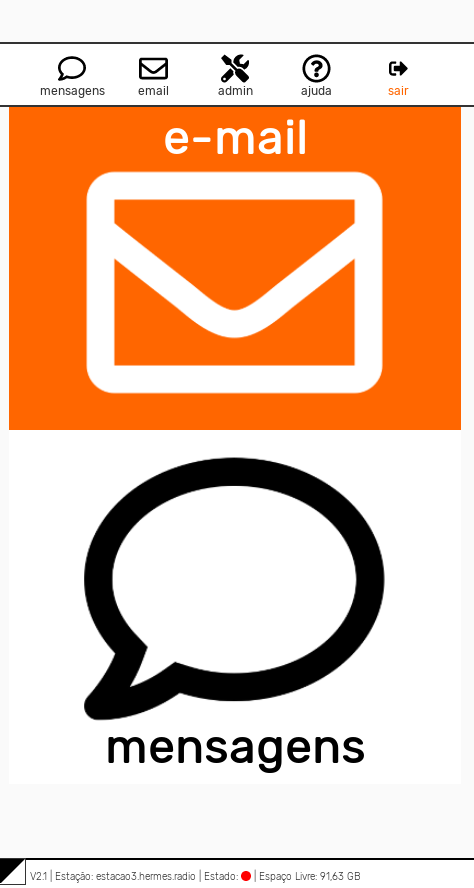
\includegraphics[width=.245\columnwidth]{gui1.png}
    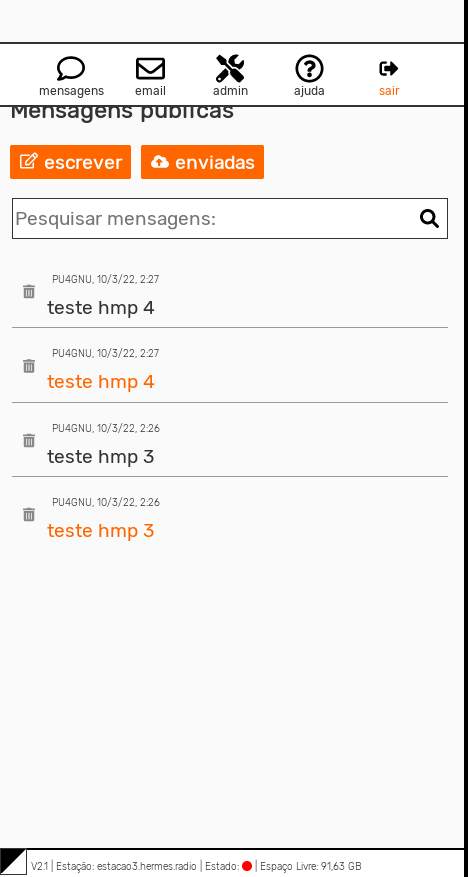
\includegraphics[width=.245\columnwidth]{gui2.png}
    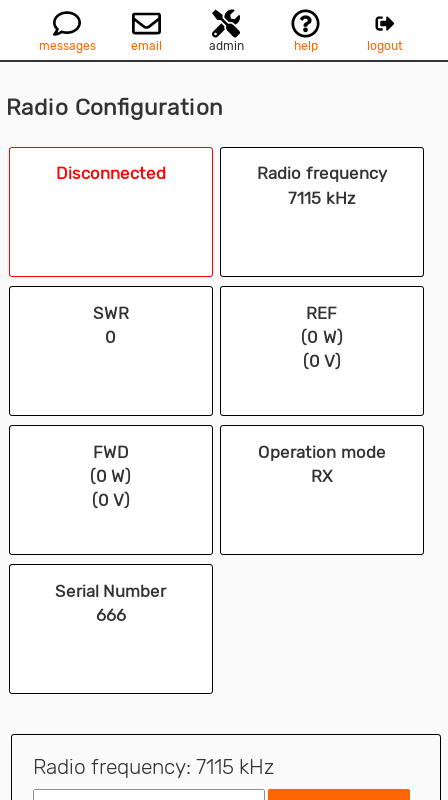
\includegraphics[width=.245\columnwidth]{gui-3.png}
    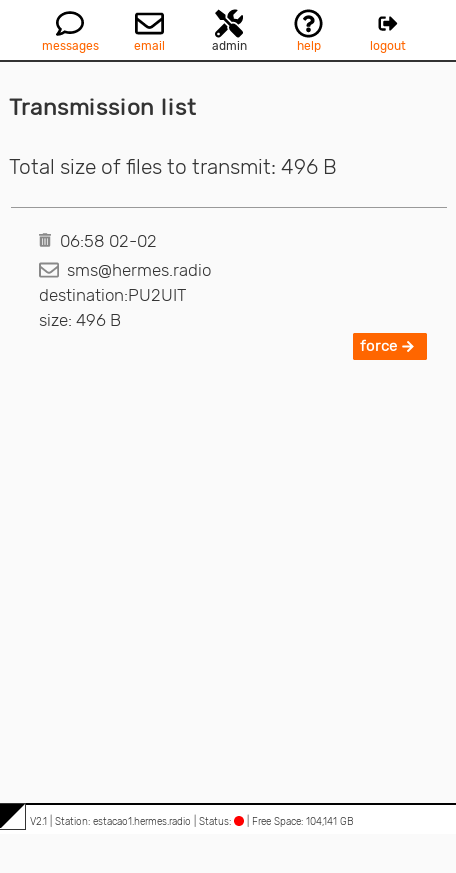
\includegraphics[width=.245\columnwidth]{gui-4.png}

  \end{center}



  \begin{block}{E-mail}
  \begin{itemize}
  \item Full e-mail stack with Postfix and Dovecot
  \item Multi-language: en, es, pt
  \item System logs, UUCP queue management
  \item Message writing / received / transmitted messages
  \item User management is tied to email user management
  \end{itemize}
\end{block}

\end{frame}


\begin{frame}{E-mail}

\begin{block}{E-mail stack}
  \begin{itemize}
  \item Full e-mail stack with Postfix, Dovecot and so on
  \item E-mail compression using uuxcomp called directly from postfix (!crmail), many headers stripped, xz compression
  \item Specific transcoding for DeltaChat audio (LPCNet) and image (VVC) messages in uuxcomp
  \item One station (called ``gateway''), which must have an Internet connection, routes the emails (uucp nodes postmap) from/to
    our email server in digital ocean
  \end{itemize}
\end{block}

\vspace{-0.15cm}
\begin{center}
%    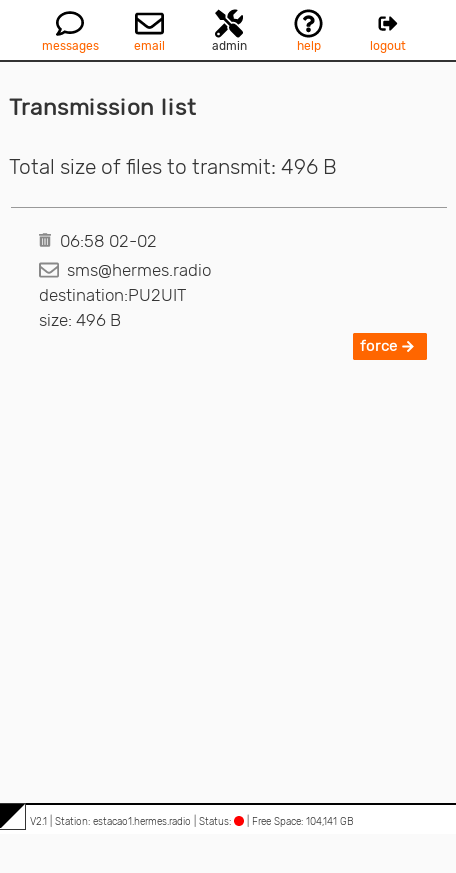
\includegraphics[width=.245\columnwidth]{gui-4.png}

\end{center}


%% add DC pictures here

\end{frame}

\begin{frame}{DeltaChat}


\begin{center}
  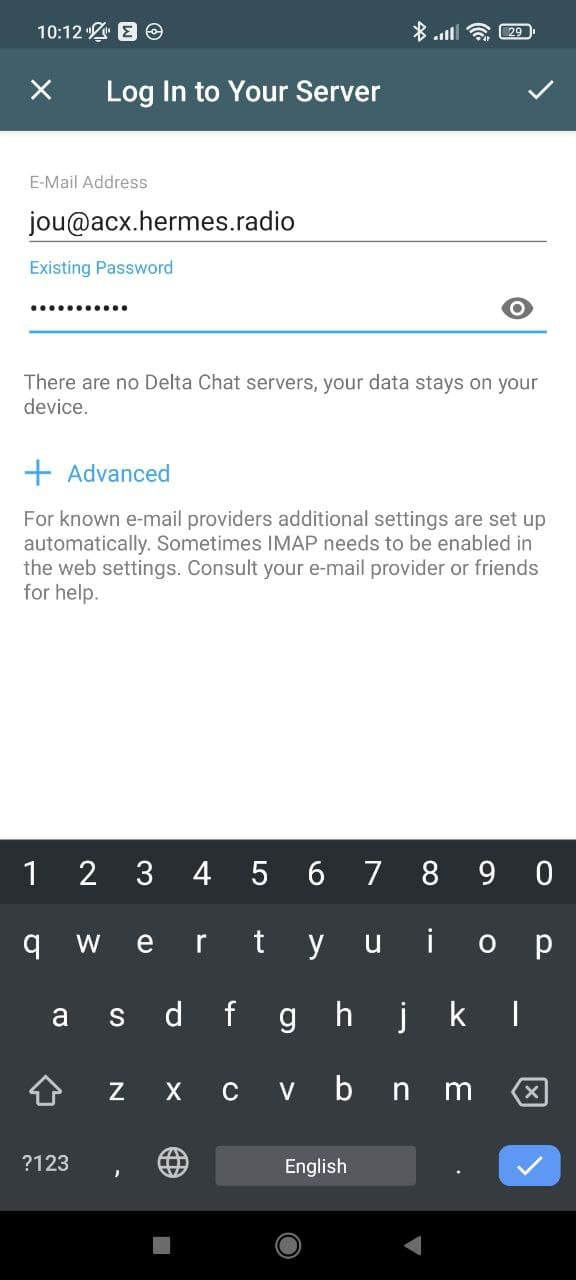
\includegraphics[width=.21\columnwidth]{dc1.jpg}
  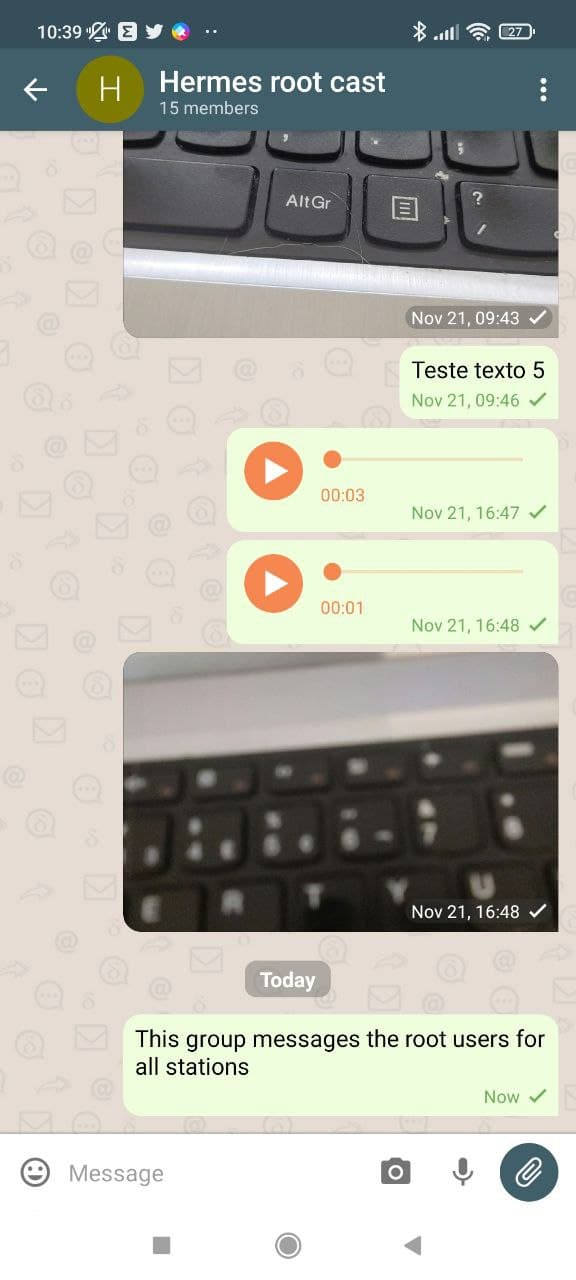
\includegraphics[width=.21\columnwidth]{dc2.jpg}
  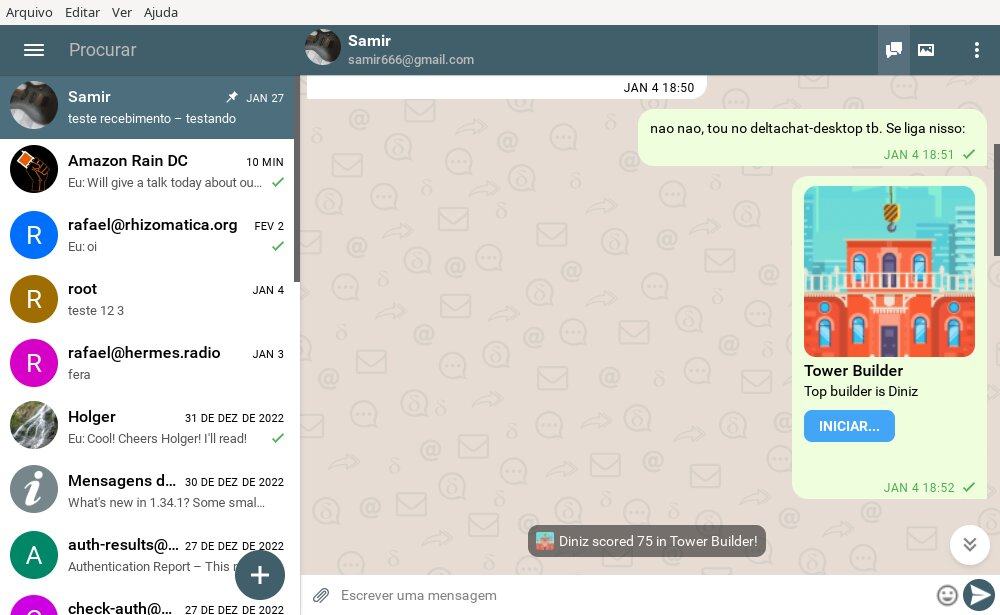
\includegraphics[width=.56\columnwidth]{webxdc.jpg}
\end{center}

\end{frame}

\begin{frame}{Near Future}

  \begin{itemize}
  \item Substiture VARA by Mercury (still lacking gear-shifting and a robust ARQ design) - HERMES will be 100\% Free Software!
  \item New Portable / WideBand HERMES version (sBitx-based)
  \item Integration to SMS and other messaging services (https://github.com/Rhizomatica/hermes-messaging/)
  \item Sensors data acquisition and transmission - binary data using paq8px compression (https://github.com/Rhizomatica/hermes-sensors/)
  \item ``Online'' GPS calibration of the Si5351 offset (using a 8-port output Si5351A)
  \item Analog SSB support in the UI (https://github.com/Rhizomatica/hermes-analog)
  \end{itemize}
\end{frame}

\begin{frame}{Future More Ahead}

  \begin{itemize}
  \item NNCP for improved security
  \item Multiple users capable (beyond P2P) MAC
  \item Adaptive bandwidth and channels selection
  \item Support synchronous communication
  \item Telephony
  \item DRM reception
  \item DRM broadcast
%  \item I'll try to avoid using IP as much as I can
  \end{itemize}

\end{frame}

\begin{frame}{HF Mobile Telephony}

\begin{center}
  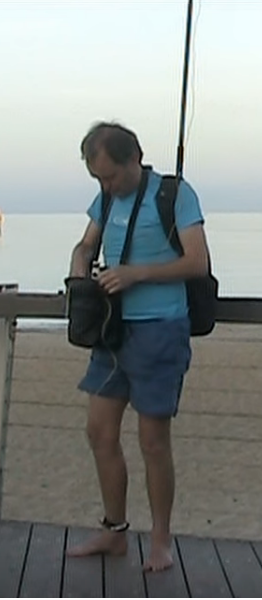
\includegraphics[width=.2\columnwidth]{mobile.png}
  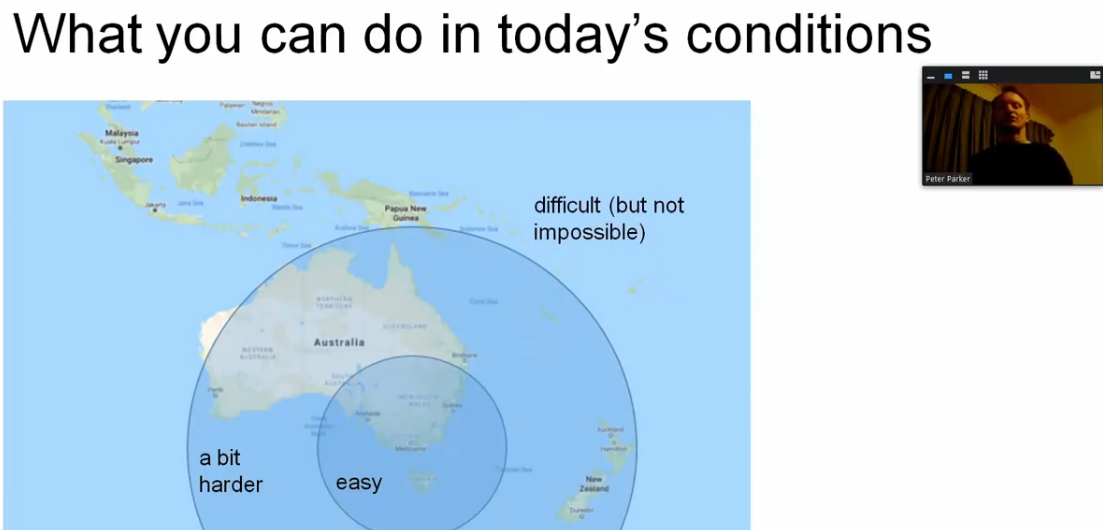
\includegraphics[width=.79\columnwidth]{mobile2.png}

\end{center}


\end{frame}


% Thank you
\begin{frame}
\centering
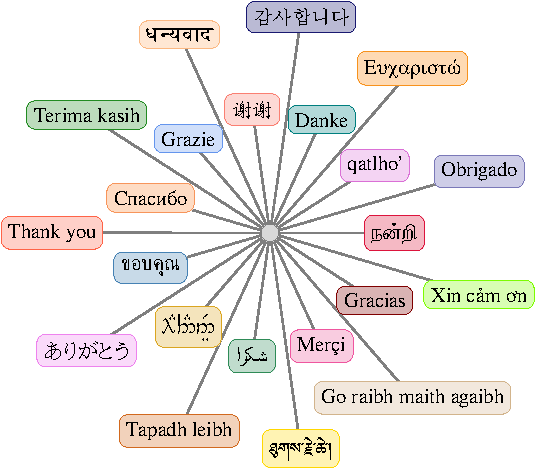
\includegraphics[width=.5\textwidth]{multiling-TQ}
\bigskip
\begin{tabular}{cl}
\multirow{3}{*}{\huge Questions?} & \textcolor{blue}{\url{rafael@rhizomatica.org}} \\
\end{tabular}

\end{frame}

\end{document}
